\PassOptionsToPackage{xetex}{xcolor}
\PassOptionsToPackage{xetex}{graphicx}
\documentclass[a4paper,landscape,headrule,footrule,xetex]{foils}

%%
%%%  Macros
%%%
\newcommand{\logo}{~}
\MyLogo{HG2052 (2020)}
%\newcommand{\Story}{\SHA{HOUN}{The Hound of the Baskervilles}}

\newcommand{\header}[3]{%
\title{\vspace*{-2ex} \Large HG2052
\\\large  Language, Technology and the Internet
\\[2ex] \Large  \emp{#2}}
\author{\blu{Francis Bond}   \\ 
\normalsize  \textbf{Division of Linguistics and Multilingual Studies}\\
\normalsize  \url{http://www3.ntu.edu.sg/home/fcbond/}\\
\normalsize  \texttt{bond@ieee.org}}
\MyLogo{HG2052 (2020)}
\date{#1}
\renewcommand{\logo}{#2}
 \hypersetup{
   pdfinfo={
     Author={Francis Bond},
     Title={#1: #2},
     Subject={HG2052: Language, Technology and the Internet},
     Keywords={Language, Technology, Internet},
     License={CC BY 4.0}
   }
 %  pdfcopyright={Copyright © Francis Bond. Creative Commons 4.0 Attribution License.}
 %  pdflicenseurl={http://creativecommons.org/licenses/by/4.0/}
 }
}


%%
%% Multilingual Stuff
%%
\usepackage[a4paper,landscape,margin=25mm]{geometry}

\usepackage{fontenc}
\usepackage{polyglossia}
\setmainlanguage{english}
\setmainfont{TeX Gyre Pagella}
%\setmainfont{Linux Libertine}
%\setmainfont{Charis SIL}
\newfontfamily{\ipafont}{Gentium}
\newcommand{\ipa}[1]{{\ipafont\selectfont #1}}
\usepackage{xeCJK}

\setCJKmainfont{Noto Sans CJK SC}
\setCJKsansfont{Noto Sans CJK SC}
%\setCJKttfont{Noto Sans CJK SC}
%\setCJKmainfont{WenQuanYi Micro Hei}
%\clearpage
%\setCJKmainfont{AR PL SungtiL GB}

\usepackage[xetex]{xcolor}
\usepackage[xetex]{graphicx}
\newcommand{\blu}[1]{\textcolor{blue}{#1}}
\newcommand{\grn}[1]{\textcolor{green}{#1}}
\newcommand{\hide}[1]{\textcolor{white}{#1}}
\newcommand{\emp}[1]{\textcolor{red}{#1}}
\newcommand{\txx}[1]{\textbf{\textcolor{blue}{#1}}}
\newcommand{\lex}[1]{\textbf{\mtcitestyle{#1}}}

\usepackage{pifont}
\renewcommand{\labelitemi}{\textcolor{violet}{\ding{227}}}
\renewcommand{\labelitemii}{\textcolor{purple}{\ding{226}}}

\newcommand{\subhead}[1]{\noindent\textbf{#1}\\[5mm]}

\newcommand{\Bad}{\emp{\raisebox{0.15ex}{\ensuremath{\mathbf{\otimes}}}}}
\newcommand{\bad}{*}

\newcommand{\com}[1]{\hfill \textnormal{(\emp{#1})}}%
\newcommand{\cxm}[1]{\hfill \textnormal{(\txx{#1})}}%
\newcommand{\cmm}[1]{\hfill \textnormal{(#1)}}%
\usepackage{amssymb}
\usepackage{relsize,xspace}
\newcommand{\into}{\ensuremath{\rightarrow}\xspace}
\newcommand{\ent}{\ensuremath{\Rightarrow}\xspace}
\newcommand{\nent}{\ensuremath{\not\Rightarrow}\xspace}
\newcommand{\tot}{\ensuremath{\leftrightarrow}\xspace}
\usepackage{url}
\usepackage[hidelinks]{hyperref}
\hypersetup{
     colorlinks,
     linkcolor={blue!50!black},
     citecolor={red!50!black},
     urlcolor={blue!80!black}
}
%\usepackage{hyperxmp}
\usepackage{url}
\newcommand{\lurl}[1]{\MyLogo{\url{#1}}}

\usepackage{mygb4e}
\let\eachwordone=\itshape
\newcommand{\lx}[1]{\textbf{\textit{#1}}}
\newcommand{\ix}{\ex\it}

\newcommand{\cen}[2]{\multicolumn{#1}{c}{#2}}
%\usepackage{times}
%\usepackage{nttfoilhead}
\newcommand{\myslide}[1]{%
\foilhead[-25mm]{\raisebox{12mm}[0mm]{\emp{#1}}}%
\leftheader{}%
\MyLogo{\logo}}

\newcommand{\mytask}[1]{%
\foilhead[-25mm]{\raisebox{12mm}[0mm]{\emp{#1}}}
\leftheader{🔍 Hi}%
\MyLogo{\logo}}

\newcommand{\myslider}[1]{\rotatefoilhead[-25mm]{\raisebox{12mm}[0mm]{\emp{#1}}}}
%\newcommand{\myslider}[1]{\rotatefoilhead{\raisebox{-8mm}{\emp{#1}}}}

\newcommand{\section}[1]{\myslide{}{\begin{center}\Huge \emp{#1}\end{center}}}

\usepackage{tcolorbox}
% \newcommand{\task}{\marginpar{\raisebox{-1ex}{\large
%       \tcbox[colframe=red,colback=white,arc=3pt]{\textbf{?}}}}}
% \newcommand{\task}{\marginpar{\raisebox{-1ex}{
%       \hspace{-0.5em}\tcbox[colframe=red,colback=white,arc=3pt]{%
%         \includegraphics[width=1.5em]{pics/detective}}}}}
\newcommand{\task}{\marginpar{\raisebox{-2ex}{
      \hspace{-0.5em}\reflectbox{\includegraphics[width=2em]{pics/detective}}}}}

\usepackage[lyons,j,e,k]{mtg2e}
\renewcommand{\mtcitestyle}[1]{\textcolor{teal}{\textsl{#1}}}
%\renewcommand{\mtcitestyle}[1]{\textsl{#1}}
\newcommand{\chn}{\mtciteform}
\newcommand{\cmn}{\mtciteform}
\newcommand{\iz}[1]{\textup{\texttt{\textcolor{blue}{\textbf{#1}}}}}
\newcommand{\con}[1]{\textsc{#1}}
\newcommand{\gm}{\textsc}
\newcommand{\cmp}[1]{{[\textsc{#1}]}}
\newcommand{\sr}[1]{\ensuremath{\langle}#1\ensuremath{\rangle}}
\usepackage[normalem]{ulem}
\newcommand{\ul}{\uline}
\newcommand{\uul}{\uuline}
\newcommand{\wl}{\uwave}
\newcommand{\vs}{\ensuremath{\Leftrightarrow}~}
%%%
%%% Bibliography
%%%
\usepackage{natbib}
%\usepackage{url}
\usepackage{bibentry}


%%% From Tim
\newcommand{\WMngram}[1][]{$n$-gram#1\xspace}
\newcommand{\infers}{$\rightarrow$\xspace}



\usepackage{rtrees,qtree}
\renewcommand{\lf}[1]{\br{#1}{}}
\usepackage{avm}
%\avmoptions{topleft,center}
\newcommand{\ft}[1]{\textsc{#1}}
\newcommand{\val}[1]{\textit{#1}}
\newcommand{\typ}[1]{\textit{#1}}
\avmfont{\sc}
%\avmvalfont{\sc}
\renewcommand{\avmtreefont}{\sc}
\avmsortfont{\it}


%%% From CSLI book
\newcommand{\mc}{\multicolumn}
\newcommand{\HD}{\textbf{H}\xspace}
\newcommand{\el}{\< \>}
\makeatother
\long\def\smalltree#1{\leavevmode{\def\\{\cr\noalign{\vskip12pt}}%
\def\mc##1##2{\multispan{##1}{\hfil##2\hfil}}%
\tabskip=1em%
\hbox{\vtop{\halign{&\hfil##\hfil\cr
#1\crcr}}}}}
\makeatletter

\newcommand{\sh}[1]{\href{https://www.arthur-conan-doyle.com/index.php?title=#1}{#1}}
\newcommand{\SHA}[2]{\href{https://www.arthur-conan-doyle.com/index.php?title=#1}{\textit{#2}}}


\header{Lecture 3}{Speech and Language Technology}





\begin{document}
\bibliographystyle{apalike}
\nobibliography{abb,mtg,nlp,ling}

\maketitle

%\include{schedule}



\myslide{Revision of Representing Language}

\begin{itemize}
\item Writing Systems
\item Encodings
\item Speech
\item Bandwidth
\end{itemize}

\myslide{Three Major Writing Systems}
\begin{itemize}
\item Alphabetic (e.g., Latin)
  \begin{itemize}
  \item  one symbol for consonant or vowel
  \item Typically 20-30 base symbols (1 byte)
  \end{itemize}
\item Syllabic (e.g., Hiragana)
  \begin{itemize}
  \item  one symbol for each syllable (consonant+vowel)
  \item Typically 50-100 base symbols (1-2 bytes)
  \end{itemize}
\item Logographic (e.g., Hanzi)
  \begin{itemize}
  \item pictographs, ideographs, sounds-meaning combinations
  \item Typically 10,0000+ symbols (2-3 bytes)
  \end{itemize}


\end{itemize}
\myslide{Computational Encoding}

\begin{itemize}
\item Need to map characters to bits
\item More characters require more space
\item Moving towards unicode for everything
\item If you get the encoding wrong, it is gibberish
\end{itemize}



\myslide{Speed is different for different modalities}
% http://en.wikipedia.org/wiki/Words_per_minute
Speed in words per minute (one word is 6 characters)
\\ (English, computer science students, various studies)

\begin{tabular}{lrlr}
  Modality & normal & peak \\ \hline 
  Reading            & 300 & 200 (proof reading)\\
  Writing              & 31 & 21 (composing) \\ 
  Speaking             & 150 & \\
  Hearing              & 150 & 210 (speeded up)  \\
  Typing               & 33  & 19 (composing) 
\end{tabular}
\begin{itemize}
\item Reading $>>$ Speaking/Hearing $>>$ Typing
  \begin{itemize}
  \item[$\Rightarrow$] Speech for input
  \item[$\Rightarrow$] Text for output
  \end{itemize}
\end{itemize}



\myslide{Speech}

\begin{itemize}
\item The need for speech representation
\item Storing sound
\item Transforming Speech
  \begin{itemize}
  \item \blu{Automatic Speech Recognition (ASR)}: sounds to text
  \item \blu{Text-to-Speech Synthesis (TTS)}: text to sound
  \end{itemize}
\item Speech technology --- the Telephone!
\end{itemize}

% Try this %%%FIXME
% \url{http://www.yellowbridge.com/onlinelit/stonelion.php}

\myslide{The need for speech}

\begin{itemize}
\item We want to be able to encode any spoken language
  \begin{itemize}
  \item What if we want to work with an unwritten language?
  \item What if we want to examine the way someone talks and don't have time to write it down?
  \end{itemize}
\item Many applications for encoding speech:
  \begin{itemize}
  \item Building spoken dialogue systems, i.e. speak with a computer (and have it speak back).
  \item Helping people sound like native speakers of a foreign language.
  \item Helping speech pathologists diagnose problems
  \end{itemize}
\end{itemize}






\myslide{What does speech look like?}




We can transcribe (write down) the speech into a phonetic alphabet. 
\begin{itemize}
\item It is very expensive and time-consuming to have humans do all the transcription.
\item To automatically transcribe, we need to know how to relate the
  audio signal to the individual sounds that we hear.
\item  We need to know:
\begin{itemize}
\item some properties of speech
\item how to measure these speech properties
\item how these measurements correspond to sounds we hear
\end{itemize}
\end{itemize}







\myslide{What makes representing speech hard?}
\begin{itemize}
\item Sounds run together, and it's hard to tell where one sound ends and another begins.
\item People say things differently from one another: 
  \begin{itemize}
  \item People have different dialects
  \item People have different sized vocal tracts 
  \end{itemize}
\item Hand written text shares similar problems
\newpage
\item People say things differently across time: What we think of as one sound is not always (usually) said the same
\item \txx{coarticulation} = sounds affect the way neighboring sounds are said
\\e.g. \eng{k} is said differently depending on if it is followed by \eng{ee} or by \eng{oo}.

\item What we think of as two sounds are not always all that different.
\\ e.g. The \eng{s} in \eng{see} is acoustically very similar to the \eng{sh} in \eng{shoe}
\end{itemize}




\myslide{Articulatory properties: How it's produced}


\begin{itemize}
\item We could talk about how sounds are produced in the vocal tract, i.e. articulatory phonetics
\begin{itemize}
\item place of articulation (where): [t] vs. [k]
\item manner of articulation (how): [t] vs. [s]
\item voicing (vocal cord vibration): [t] vs. [d]
\end{itemize}
\item But unless the computer is modeling a vocal tract, we need to know acoustic properties of speech which we can quantify.
\end{itemize}





\myslide{Measuring sound}

\begin{itemize}
\item Sound is actually a continuous wave
\item We store data at each discrete point, in order to capture the general pattern of the sound
\item \blu{Sampling Rate:} how many times in a given second we extract a moment of sound; measured in samples per second
\item Sound is continuous, but we prefer to store data in a discrete manner.
\end{itemize}

\myslide{Signal sampling representation.}
\MyLogo{\url{https://en.wikibooks.org/wiki/A-level_Computing/AQA/Problem_Solving,_Programming,_Data_Representation_and_Practical_Exercise/Fundamentals_of_Data_Representation/Sampled_sound}}
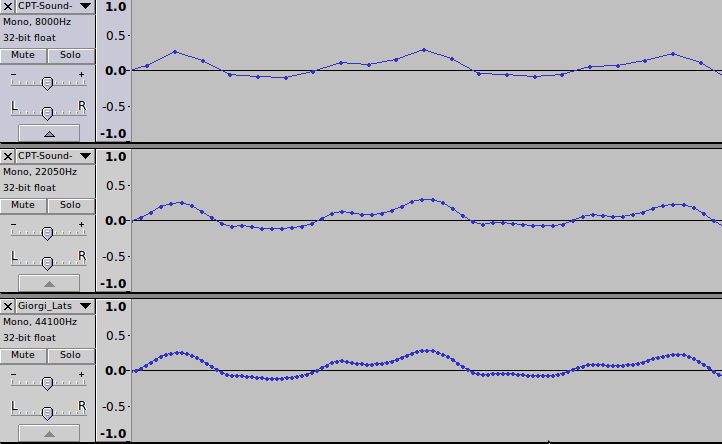
\includegraphics[height=0.9\textheight]{../pics/CPT-Sound-SampleRate-3way-Comparison.png}

Comparison of a sound sample recorded at 8kHz, 22kHz and 44kHz.

\myslide{Sampling rate}


The higher the sampling rate, the better quality the recording ... but the more space it takes. 

\begin{itemize}
\item Speech needs at least 8000 samples/second, but most likely 16,000 or 22,050 Hz will be used nowadays.
\item The rate for CDs is 44,100 samples/second (or Hertz (Hz))
\end{itemize}
Now, we can talk about what we need to measure, \ldots









\myslide{Acoustic properties: What it sounds like}
\begin{itemize}
\item \blu{Sound waves}: ``small variations in air pressure that occur very rapidly one after another''
\item The main properties we measure:
  \begin{itemize}
  \item \blu{speech flow}:  rate of speaking, number and length of pauses (seconds)
  \item \blu{amplitude} (loudness): amount of energy (decibels)
  \item \blu{frequency}: how fast the sound waves are repeating (cycles per second, i.e. Hertz)
    \begin{itemize}
    \item \blu{pitch}:  how high or low a sound is
    \item In speech, there is a fundamental frequency, or pitch, along with higher-frequency overtones.
    \end{itemize}
  \end{itemize}
\end{itemize}

Researchers also look at things like intonation, i.e., the rise and fall in pitch



\myslide{Speech Sample}
\noindent\includegraphics[width=\textwidth]{../pics/BushAPlan.eps}


Pitch track, transcription, spectogram and audio waveform.



\myslide{Measurement-sound correspondence}


\begin{itemize}
\item  How dark is the picture? $\rightarrow$ How loud is the sound?
  \begin{itemize}
  \item We measure this in decibels.
  \end{itemize}
\item Where are the lines the darkest? $\rightarrow$  Which frequencies are the loudest and most important?
  \begin{itemize}
  \item We can measure this in terms of Hertz, and it tells us what the vowels are.
  \end{itemize}

\item Speech signals are very different from text.
  \begin{itemize}
  \item No segmentation into words!
  \end{itemize}
\end{itemize}




\myslide{Applications of speech encoding}


\begin{itemize}
\item Mapping sounds to symbols (alphabet), and vice versa, has some very practical uses.
  \begin{itemize}
  \item \blu{Automatic Speech Recognition (ASR)}: sound to text
  \item \blu{Text-to-Speech Synthesis (TTS)}: text to sound
  \end{itemize}
\item These are not easy tasks.
\item Text-to-Speech Synthesis is somewhat easier.
\end{itemize}

\section{Automatic Speech Recognition (ASR)}

\myslide{Automatic Speech Recognition (ASR)}

\begin{itemize}
\item Automatic speech recognition = process by which the computer maps a speech signal to text.
\item Uses/Applications:
  \begin{itemize}
  \item Dictation
  \item Dialogue systems
  \item Telephone conversations
  \item People with disabilities – e.g. a person hard of hearing could use an ASR system to get the text (closed captioning)
  \item Spying (many agencies run ASR on phone conversations and search for keywords)
  \item Indexing audio data
  \end{itemize}
\end{itemize}








\myslide{Steps in an ASR system}

\begin{enumerate}
\item Digital sampling of speech
\item \blu{Acoustic signal processing} = converting the speech samples into particular measurable units
\item Recognition of sounds, groups of sounds, and words 
\end{enumerate}

May or may not use more sophisticated analysis of the utterance to
help. e.g., a [t] might sound like a [d], and so word information
might be needed (more on this later)









\myslide{Kinds of ASR systems}


Different kinds of systems, with an accuracy-robustness tradeoff: 

\begin{itemize}
\item \blu{Speaker dependent:} works for a single speaker
\item \blu{Speaker independent:} works for any speaker of a given variety of a language, e.g. American English
\item A common type of system starts general, but learns  
\begin{itemize}
\item \blu{Speaker adaptive} = start as independent but begin to adapt to a single speaker to improve accuracy
\item Adaptation may simply be identifying what type of speaker a
  person is and then using a model for that type of speaker
\item Or if it can get verification of it's hypothesis (e.g. did you
  click the search result), then it can add it as training data
\end{itemize}
\end{itemize}








\myslide{Kinds of ASR systems}

\begin{itemize}
\item Differing sizes and types of vocabularies
\begin{itemize}
\item from tens of words to tens of thousands of words
\item normally very domain-specific, e.g., flight vocabulary
\end{itemize}
\item continuous speech vs. isolated-word systems:
\begin{itemize}
\item \blu{continuous speech systems} = words connected together and not separated by pauses
\item \blu{isolated-word systems} = single words recognized at a time, requiring pauses to be inserted between words 
  \begin{itemize}
  \item easier to find the endpoints of words
  \item harder to use
  \end{itemize}
\end{itemize}
\end{itemize}


\myslide{Word Error Rate in Speech Recognition}

\begin{itemize}
\item The first successful wide spread testing in NLP
  \begin{itemize}
  \item Compare your output to a reference
  \item Calculate the number of substitutions, deletions and insertions to make them match
(Minimum Edit Distance)
  \item Normalize by dividing by the length of the reference\\[2ex]
    {\Large
    $\begin{array}{lcr}
      WER = \frac{S+D+I}{N}
    \end{array}$
}
  \end{itemize}

\item 
  \begin{tabular}[t]{llllllllll}
    Reference: & I &want &to &recognize&  & &speech & today \\
    System:    & I &want &   &wreck    &a &nice &peach & today\\
    Eval:      &   &     & D   & S       & I & I & S \\
  \end{tabular}
\item $WER=\frac{2+1+2}{6}=0.83$
% (/ 5 6.0) 0.8333333333333334
\end{itemize}


\myslide{Some properties of WER}

\begin{itemize}
\item Correlates well with the task
\item Reducing WER is always a good thing
\item A WER of 0 implies perfect results
  \\ (assuming the reference is correct)
\item $WER < .95$ considered the minimum to be useful
\item Competitions were held to see who could get the lowest WER
  \begin{itemize}
  \item Speech Recognition had 10 years of rapid improvement
  \item It has slowed down now
  \end{itemize}
\end{itemize}


\myslide{How good are the systems?}

  \begin{tabular}{lrrr}
    Task & Vocab & WER (\%) & WER  (\%) adapted \\ \hline
    Digits & 11 & 0.4 & 0.2 \\
    Dialogue (travel) & 21,000 & 10.9 & --- \\
    Dictation (WSJ) & 5,000 & 3.9 & 3.0 \\
    Dictation (WSJ) & 20,000 & 10.0 & 8.6 \\
    Dialogue (noisy, army) & 3,000 & 42.2 & 31.0 \\
    Phone Conversations & 4,000 & 41.9 & 31.0 \\
  \end{tabular}

Results of various DARPA competitions (from Richard Sproat's slides, 2012)

Improvements in machine learning (\txx{deep learning}) have
further reduced errors

\begin{itemize}
\item A combination of learning a combined model and better training data
\\
\href{https://ai.googleblog.com/2017/12/improving-end-to-end-models-for-speech.html}{Improving
  End-to-End Models For Speech Recognition} (Google AI Blog 2017)
\\ WER of 5.6\% (16\% relative improvement over 6.7\%)
\begin{itemize}
\item
  \href{https://ai.googleblog.com/2018/08/Multilingual-Google-Assistant.html}{Teaching
    the Google Assistant to be Multilingual} (2018)
\item
  \href{https://ai.googleblog.com/2018/04/looking-to-listen-audio-visual-speech.html}{Looking
    to Listen: Audio-Visual Speech Separation} (2018)
\end{itemize}
\end{itemize}



\myslide{Why is it so difficult?}
\begin{itemize}
\item Speaker variability
  \begin{itemize}
  \item Gender
  \item Dialect/Foreign Accent
  \item Individual Differences: Physical differences; Language differences (idiolect)‏
  \end{itemize}
\item Many, many rare events
  \begin{itemize}
  \item 300 out of 2,000 diphones in the core set for the AT\&T NextGen system occur only once in a 2-hour speech database
  \end{itemize}
\end{itemize}
\myslide{Rare events are \blu{frequent}}
\begin{itemize}
\item Collect about 10,000,000 character 4-grams, from English
  newswire text, merging upper and lower case — 60 distinct characters
  including space.
\item 197,214 lines of text.
\item Of these, 14,317 (7\%) contain at least one 4-gram that only occurs once in 10,000,000.
\item Increase it to 5-grams: 21\% of lines contain contain at least
  one 5-gram that only occurs once in 10,000,000.
\end{itemize}

\myslide{What is an $n$-gram?}
\begin{itemize}
\item An \blu{$n$-gram} is chunk of $n$ things: most often words, but could
  be characters, letters, morphemes, stems, \ldots
 \item Approximation of language: information in $n$-grams tells us something about language, but doesn't capture the structure
 \item Efficient: finding and using every, e.g., two-word collocation in a text is quick and easy to do
 \item $n$-grams help a variety of NLP applications, including word prediction
   \begin{itemize}
   \item We can predict the next word of an utterance, based on the previous 
     % $n - 1$ words
   \end{itemize}
 \item \textit{unigram, bigram, trigram, 4-gram, \ldots}
\end{itemize}
\section{Text-to-Speech Synthesis (TTS)}

\myslide{Text-to-Speech Synthesis (TTS)}
\begin{itemize}
\item Could just record a voice saying phrases or words and then play back those words in the appropriate order.
\item This won't work for, e.g., dialogue systems where speech is generated on the fly.
\item Or can break the text down into smaller units
  \begin{enumerate}
  \item Convert input text into phonetic alphabet (\emp{ambiguous} mapping)
  \item Synthesize phonetic characters into speech 
  \end{enumerate}
\item  To synthesize characters into speech, people have tried:
  \begin{itemize}
  \item using a model based on frequencies, the loudness, etc.
  \item using a model of the vocal tract and human speech production
  \end{itemize}
\end{itemize}

\myslide{Demo of Festival}

\blu{Festival} -- a current  system:
\\ \url{http://www.cstr.ed.ac.uk/projects/festival/onlinedemo.html}

\begin{description}
\item [HTS] - a statistical parametric approach (both the 2005 and 2007 systems)
\item [Unit] - standard unit selection concatenative approach
\\ look for variable-length units in an
annotated database of speech, and select them on the basis of various
features including desired phoneme sequence and prosody.
Units can be individual phones, diphones, half-phones, syllables, morphemes, words, phrases, and sentences. 
\item [Diphone] - single instance diphone concatenation
\\      (the previous TTS generation technology, from mid 1980's to mid 1990's). 
\end{description}

\myslide{Two steps in a TTS system}

\begin{enumerate}
\item Linguistic Analysis
  \begin{itemize}
  \item Sentence Segmentation
  \item Abbreviations: \eng{Dr Smith lives on Nanyang Dr. She is \ldots}
  \item Word Segmentation: 
    \begin{itemize}
    \item 森山 前 日銀 総裁 \jpn{Moriyama zen Nichigin Sousai}
    \item[\Bad]  森山 前日 銀 総裁 \jpn{Moriyama zennichi gin Sousai}
      \end{itemize}
    \end{itemize}
\item Speech Synthesis
  \begin{itemize}
  \item Find the pronunciation
  \item Generate sounds
  \item Add intonation
  \end{itemize}
\end{enumerate}

\myslide{Linguistic Analysis (cont)}

\begin{itemize}
\item Acronyms: \eng{NTU, NATO}
\item Numbers: \eng{666 green bottles; They were branded with 666.}
\item Senses: \eng{Star Wars IV; IV drip} (``four vs ``intravenous'')
  \\ \eng{Are you content with the content?}
\\ \eng{The bandage was wound round the wound.}
\\ \eng{Polish polish should be used.}
\item Inflection:
  \begin{description}
  \item[statement] falling intonation
  \item[question] rising intonation
  \item[{\ldots}]
  \end{description}
\end{itemize}

\myslide{Segmental durations:}
\begin{itemize}
\item Every sound has to have some time assigned to it
\item Other things being equal:
  \begin{itemize}
  \item Vowels tend to be longer than consonants
  \item Stressed segments tend to be longer than unstressed segments
  \item Accented segments tend to be longer than unaccented segments
  \item Final segments tend to be longer than non-final segments
  \item Segments have different inherent durations: 
    \\ /ee/ in \eng{keep} is generally longer than /i/ in \eng{kip}
    \end{itemize}
  \end{itemize}
\myslide{Synthesizing Speech: Analysis}
  \begin{itemize}
  \item From linguistic analysis we have:
    \begin{itemize}
    \item A set of sounds to be produced
    \item   Associated durations
    \item   Associated fundamental frequency information
    \item   Possibly other things:
          \begin{itemize}
            \item Amplitude
           \item  Properties of the vocal production
          \end{itemize}
        \end{itemize}
      \item Now we are ready to synthesize speech
  \end{itemize}



\myslide{Speech Synthesis}
  \begin{itemize}
  \item \blu{Articulatory Synthesis:} Attempt to model human articulation.
  \item \blu{Formant Synthesis:} Bypass modeling of human articulation, and model acoustics directly.
  \item \blu{Concatenative Synthesis:} Synthesize from stored units of actual speech
  \end{itemize}
  

\myslide{Human Vocal Apparatus}
\begin{center}
  \noindent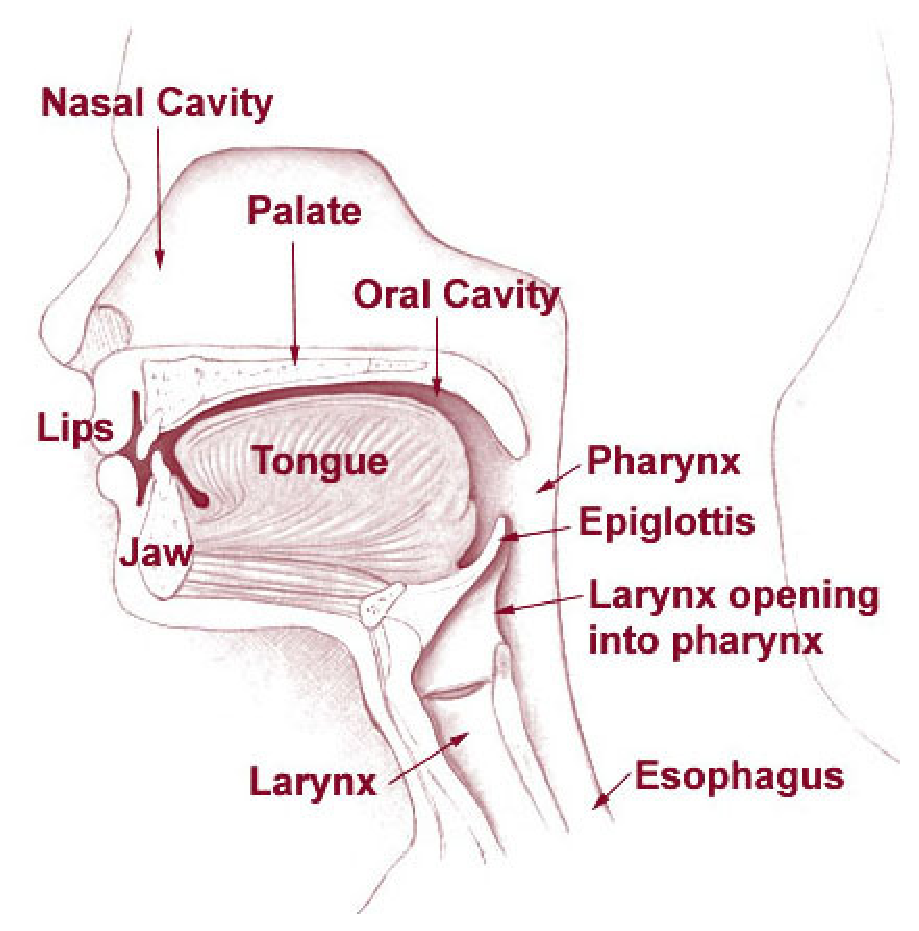
\includegraphics[height=0.8\textheight]{../pics/Illu01_head_neck.eps}
\end{center}

{\small \url{http://en.wikipedia.org/wiki/File:Illu01_head_neck.jpg}}

\myslide{Articulatory Synthesis}
\begin{itemize}
\item Articulatory synthesizers will produce a set of instructions to articulators (larynx, velum, tongue body, tongue tip, lips, jaw)
  \begin{itemize}
  \item This will produce a sequence of articulatory configurations
  \item From acoustic theory one derives the acoustics of each configuration
  \end{itemize}
\item   Articulatory synthesis is very hard: 
  \begin{itemize}
  \item We do not fully understand how the articulators move
  \item We do not fully understand how to model the acoustics
  \end{itemize}
\end{itemize}

\myslide{Synthesizing Speech}
\MyLogo{\url{http://www.popsci.com/technology/article/2011-07/moaning-mouth-bot-learns-croon-even-creepier-ever}}

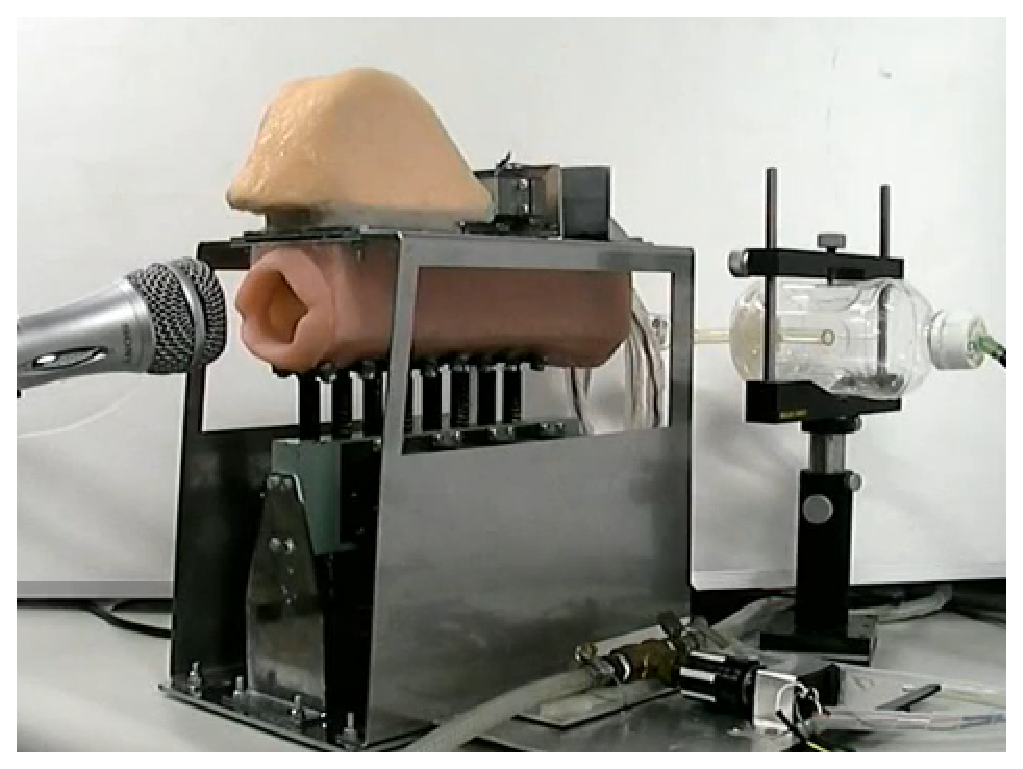
\includegraphics[height=\textheight]{../pics/mouth.eps} %(IEEE Spectrum)
  % \myslide{Synthesizing Speech}

% \begin{itemize}
% \item In some sense, TTS really is the reverse process of ASR
%   \begin{itemize}
%   \item Since we know what frequencies correspond to which vowels, we can play those frequencies to make it sound like the right vowel.
%   \item However, sounds are always different (across time, across speakers)
%   \end{itemize}
% \item One way to generate speech is to have a database of speech and to use the diphones, i.e., two-sound segments, to generate sounds.
% \item Diphones help with the context-dependence of sounds
% \end{itemize}

\myslide{Formant synthesis}
\begin{itemize}
\item Formant synthesizers attempt to model the acoustics directly by means of rules that capture the change of acoustic parameters over time.
\item This is easier than articulatory synthesis but is still hard
\end{itemize}


\myslide{Concatenative synthesis}
\begin{itemize}
\item Record real speech from a single talker
\item Segment the speech so that we know where the individual sounds are
\item Either:
  \begin{itemize}
  \item Preselect a database of units: diphone, polyphone synthesis
  \item Select the best unit at runtime: unit-selection synthesis
    \begin{itemize}
    \item At synthesis time, appropriate units are selected from the database and concatenated
      \begin{itemize}
      \item Some smoothing between units is generally necessary
      \item Units need to be stretched or compressed to fit within the specified duration
      \end{itemize}
    \item Intonation, and amplitude information is added, and the system is sent for synthesis.
    \end{itemize}
  \end{itemize}
\end{itemize}

\myslide{Prosody of Emotion}

\begin{itemize}
\item Excitement: Fast, very high pitch, loud
\item Hot anger: Fast, high pitch, strong, falling accent, loud
\item Fear: Jitter
\item Sarcasm: Prolonged accent, late peak
\item Sad: Slow, low pitch
\end{itemize}

\begin{quote}
  The main determinant of ``naturalness'' in speech synthesis is not
  ``voice quality'', but natural-sounding prosody (intonation and
  duration) 
  \begin{flushright}
    Richard Sproat
  \end{flushright}
\end{quote}

\myslide{It's hard to be natural} When trying to make synthesized
speech sound natural, we encounter the same problems that make
speech encoding hard:

\begin{itemize}
\item The same sound is said differently in different contexts.
\item Different sounds are sometimes said nearly the same.
\item Different sentences have different intonation patterns. 
\item Lengths of words vary depending on where in the sentence they are spoken. 
    \begin{enumerate}
    \item The \blu{car} crashed into the tree.
    \item It's my \blu{car}.
    \item \blu{Cars}, trucks, and bikes are vehicles.
    \end{enumerate}
  \end{itemize}






\myslide{Speech to Text to Speech}

If we convert speech to text and then back to speech, it should sound the same.
\begin{itemize}
\item  But at the conversion stages, there is information loss.
\item To avoid this loss would require a lot of memory and knowledge about what exact information to store.
\item The process is thus irreversible.
\item In fact, people can't say the same sentence exactly the same way either!
\end{itemize}

\myslide{TTS Applications}
Any situation where you need information, but can't access it visually:

\begin{itemize}
\item Access to information for the blind
\item Access to email, news, stock quotes \ldots over the phone
\item Directions to drivers
\item Spoken dialog systems where it is not practical to prerecord everything
\item Informational content – e.g. NOAA Weather Radio – where it would be expensive to have a human read all the announcements.
\end{itemize}
\section{Mediums of Communication}
\myslide{Mediums of Communication}

\begin{itemize}
\item Different mediums of communication 
  \begin{itemize}
  \item affect the language used within them
  \item may affect our social organization
  \end{itemize}
\item We will analyze them compared to speech/text
  \begin{itemize}
  \item More fine grained analyses exist \citep{Herring:2007}
  \end{itemize}
\end{itemize}


\myslide{The Telephone}

\begin{tabular}{ll}
  \textbf{Speech like} & \textbf{Text like} \\ \hline
  \blu{time bound} & space bound \\
  \blu{spontaneous} & contrived \\
  face-to-face & \blu{visually decontextualized} \\
  \blu{loosely structured} & elaborately structured \\
  \blu{socially interactive} & factually communicative \\  
  \blu{immediately revisable} & repeatedly revisable  \\
  \blu{prosodically rich} & graphically rich \\
\end{tabular}

\begin{itemize}
\item Technology enabling a new modality of communication
\item Speech-like but not exactly speech
\item Analysis from \citet{Crystal:2006}
\end{itemize}

\myslide{Phone Schema}

\begin{enumerate} \addtolength{\itemsep}{-1ex}
\item Greeting/Introduction
  \\ \eng{Hello.  This is $\sim$.  Thank you for calling $\sim$.}
  \\ \textbf{jpn}: \eng{moshi-moshi}; \textbf{kor}: \eng{yeobo seyo}
\item Connecting:  \eng{May I speak to $\sim$.  I'll put you through.}
\item Meta-requests
 \\ \eng{Can you call me back? I think we have a bad connection.
\\   Can you please hold for a minute? I have another call.}
%Could you speak up a little please?
%# Can you speak a little slower please. My English isn't very strong.
\item Taking a message
\\ \eng{Can I ask who's calling?  Would you like to leave a message?}
\item Finishing:
\eng{Thanks for calling. Bye for now.}
\end{enumerate}
\begin{quote}
  \blu{Conventions for dealing with the new technology}
\end{quote}

% Introducing yourself
% This is Ken.
% Ken speaking

% Asking who is on the telephone
% Excuse me, who is this?
% Can I ask who is calling, please?
% Asking for Someone
% Can I have extension 321? (extensions are internal numbers at a company)
% Could I speak to...? (Can I - more informal / May I - more formal)
% Is Jack in? (informal idiom meaning: Is Jack in the office?
% Connecting Someone
% I'll put you through (put through - phrasal verb meaning 'connect')
% Can you hold the line? Can you hold on a moment?
% How to reply when someone is not available
% I'm afraid ... is not available at the moment
% The line is busy... (when the extension requested is being used)
% Mr Jackson isn't in... Mr Jackson is out at the moment...
% Taking a Message
% Could (Can, May) I take a message?
% Could (Can, May) I tell him who is calling?
% Would you like to leave a message? 

\myslide{Affects of the telephone}

\begin{itemize}
\item The telephone (and telegraph) had a big effect on independence
  of subsidiaries in large international organizations \citep{Parkinson:1958}
  \begin{itemize}
  \item Central offices could micromanage people in the field
  \item More centralization, less local flexibility 
  \end{itemize}
\end{itemize}

\myslide{What do you use?}

Results of the Media Usage Survey

\myslide{Acknowledgments and References}

\begin{itemize}
\item Many slides on speech technology adapted from Richard Sproat's L270: 
  \\ \url{http://catarina.csee.ogi.edu/L270/}
\item \bibentry{Crystal:2006}
\item \bibentry{Herring:2007}
\item \bibentry{Parkinson:1958}
\end{itemize}




%%
%% Future
%%

\end{document}


%%% Local Variables: 
%%% coding: utf-8
%%% mode: latex
%%% TeX-PDF-mode: t
%%% TeX-engine: xetex
%%% End: 
